\documentclass[10pt]{article}
\usepackage[margin=1in]{geometry}
\usepackage[T1]{fontenc}
\usepackage{mathptmx}
\usepackage{courier}
\usepackage{microtype}
\usepackage{amsmath,amssymb}
\usepackage{booktabs}
\usepackage{graphicx}
\usepackage{xcolor}
\usepackage[numbers,sort&compress]{natbib}
\usepackage[hidelinks]{hyperref}
\usepackage{caption}
\captionsetup{font=small,labelfont=bf}

\newcommand{\ctx}{\textsc{ctx\_gain}}
\newcommand{\bpb}{bpb}

\title{Is the Hierarchy Doing Anything?\\Main-Network Collapse in Hierarchical Byte-Level Language Models}
\author{Anonymous Authors}
\date{}

\begin{document}
\maketitle

\begin{abstract}
Hierarchical byte-level language models such as H-Net compress a byte sequence into chunks,
process the chunks with a large \emph{main network}, and decode back to bytes, with a residual
path from encoder to decoder. We show that this design has a silent failure mode: the main
network can \emph{collapse} to an almost input-independent output while the encoder--residual--decoder
path alone does the language modelling. We measure this with a simple diagnostic, \ctx{}: the
increase in validation bits-per-byte (\bpb) when the main network's output is replaced by its
per-sequence mean. In $\sim$70 GPU training runs of 100--150M-parameter models on FineWeb-Edu bytes,
both in our re-implementation and in the official H-Net code, every model with static or
non-learned chunk boundaries collapsed (\ctx{}$\le 0.02$), while H-Net's learned dynamic
chunking usually kept the main network in use. In this regime, H-Net's advantage over
fixed-stride chunking (0.11 \bpb{} in the official code) is explained by \emph{whether the hierarchy
is used at all}, and \bpb{} correlates strongly with \ctx{} across runs ($r=-0.82$). Collapse is
also seed-dependent for H-Net itself (3/20 seeds in our re-implementation; one of three official
seeds was only partially alive and 0.1 \bpb{} worse). Three straightforward anti-collapse
interventions did not revive static chunking, nor did seven new chunking mechanisms we
designed. A new routing feature that anticipates next-byte difficulty removed collapse in
20/20 seeds but its improvement over H-Net (1.322 vs.\ 1.333 \bpb) is not statistically
significant. We recommend reporting \ctx{} (or an equivalent bypass check) and multiple seeds
for any hierarchical byte-level model.
\end{abstract}

\section{Introduction}

Tokenizer-free language models operate directly on bytes and recover efficiency by
hierarchy: an inexpensive \emph{encoder} works at byte resolution, a large \emph{main network}
works on a shorter sequence of chunks, and a \emph{decoder} maps chunk-level states back to
byte predictions \citep{nawrot2021hourglass,yu2023megabyte,slagle2024spacebyte,pagnoni2024blt,hwang2025hnet}.
H-Net \citep{hwang2025hnet} learns where to place chunk boundaries end-to-end (``dynamic
chunking'') and reports that this outperforms fixed or heuristic chunking.

We set out to design a better dynamic chunking mechanism and instead found that, at the scale we
could afford, the decisive variable was not \emph{where} chunks are placed but \emph{whether the main network
is used at all}. Hierarchical byte LMs contain a residual path from encoder to decoder; when the
encoder and decoder can model local structure themselves, the main network can degenerate into
an approximately constant vector without the training loss revealing it. The model then looks
like a normal, reasonably good byte-level LM.

\paragraph{Contributions.}
\begin{itemize}
\item A cheap diagnostic, \ctx{} (Section~\ref{sec:diag}), and a complementary inference-time
  test (changing the compression of a trained model), which expose a bypassed hierarchy.
\item Evidence from a re-implementation and from the official H-Net code that static chunking
  collapses in every run, while H-Net's learned routing usually prevents collapse; H-Net's
  advantage over fixed-stride chunking tracks main-network use (Section~\ref{sec:results}).
\item Seed-level statistics (20 seeds per arm) showing that collapse is stochastic even for H-Net.
\item Negative results for seven new chunking mechanisms and three anti-collapse interventions,
  and a null result (with 20 seeds) for an anticipatory routing feature
  (Sections~\ref{sec:negative}--\ref{sec:anticip}).
\end{itemize}

\section{Background: H-Net and dynamic chunking}
\label{sec:background}

A one-stage H-Net \citep{hwang2025hnet} maps bytes $x_{1:L}$ to encoder states $h_{1:L}$. A
routing module predicts boundary probabilities $p_t = \tfrac12(1-\cos(W_q h_{t-1}, W_k h_t))$;
positions with $p_t\ge 0.5$ start a new chunk, and their states form the main network's input
sequence $z_{1:M}$ ($M\approx L/N$ for a target compression $N$, encouraged by a
load-balancing loss). The main network's outputs $y_{1:M}$ are \emph{de-chunked} with an
exponential moving average whose rate is $p$, broadcast back to bytes, multiplied by a
straight-through confidence term \citep{bengio2013ste}, added to a residual projection of
$h$, and decoded. The encoder and decoder use Mamba-2 \citep{dao2024mamba2} layers in the
official release; the main network is a Transformer. Gradients reach the router only through
the EMA rate and the straight-through term.

\section{Diagnosing a bypassed hierarchy}
\label{sec:diag}

\paragraph{\ctx{}.} For a trained model, we evaluate validation \bpb{} twice on the same
batches: normally, and with the main network's output $y_{1:M}$ replaced by its mean over the
$M$ chunks of each sequence (keeping its average contribution, removing all chunk-specific
information). We define
\[
\ctx{} = \bpb_{\text{mean-replaced}} - \bpb_{\text{normal}} .
\]
A model whose decoder ignores the main network's \emph{content} has $\ctx{}\approx 0$, even if
the main network contributes a useful constant bias (zeroing $y$ instead would conflate the two).
The test costs two evaluation passes and needs no retraining. We call a run \emph{collapsed}
when $\ctx{}\le 0.05$; the threshold is arbitrary, but the distribution is clearly separated
in practice (Figure~\ref{fig:scatter}).

\paragraph{Changing the compression after training.} A second, independent signature: if the
main network is bypassed, the model's \bpb{} should be insensitive to how bytes are chunked at
inference. We vary the stride (fixed chunking) or the boundary threshold (H-Net) of a trained
model and measure \bpb{} (Figure~\ref{fig:dial}).

\section{Experimental setup}
\label{sec:setup}

\paragraph{Data.} FineWeb-Edu \citep{penedo2024fineweb} \texttt{sample-10BT}, shards 0--1, as raw
UTF-8 bytes (6.9\,GB train; the last 1\% of documents, 71\,MB, for validation). Each run trains on
9{,}000 steps $\times$ 32 sequences $\times$ 2{,}048 bytes $\approx$ 590M bytes, and is evaluated
on 100 batches of the validation set; the same seed implies the same data order in every arm.

\paragraph{Re-implementation (``ours'').} A pure-PyTorch 1-stage hierarchy: byte embedding;
encoder of 4 Transformer layers ($d{=}512$, 128-byte sliding-window attention); a chunker;
main network of 12 Transformer layers ($d{=}768$, full causal attention); de-chunking;
residual; decoder of 4 Transformer layers ($d{=}512$, 128-byte window); $\approx$150M parameters.
AdamW, learning rate $10^{-3}$ with cosine decay and 1k warmup steps, main-network learning rate
$\times 0.3$ (analogous to H-Net's per-stage multipliers), bf16, target compression $N{=}4$.
All chunkers pass a causality test that perturbs future bytes and checks that earlier logits are
unchanged.

\paragraph{Official code.} The released \texttt{hnet} package, unmodified except for routing
overrides for the ``fixed'', ``random'' and anticipatory variants: Mamba-2$\times$4 encoder and
decoder ($d{=}512$), Transformer$\times$12 main network ($d{=}768$, FFN 2048), $\approx$100M
parameters, the official load-balancing loss ($\alpha{=}0.03$, $N{=}4$) and per-stage learning-rate
multipliers $[2.0, 1.0]$ on a base rate of $5\cdot10^{-4}$. Identical data, steps and evaluation.
``Fixed'' forces a boundary every 4 bytes (the EMA then reduces to repetition and the
straight-through factor to 1).

\paragraph{Compute.} H100 80GB PCIe (some official runs on A100), one or two runs per GPU, rented
on demand; $\sim$1\,h per run.

\section{Results}
\label{sec:results}

\begin{figure}[t]
\centering
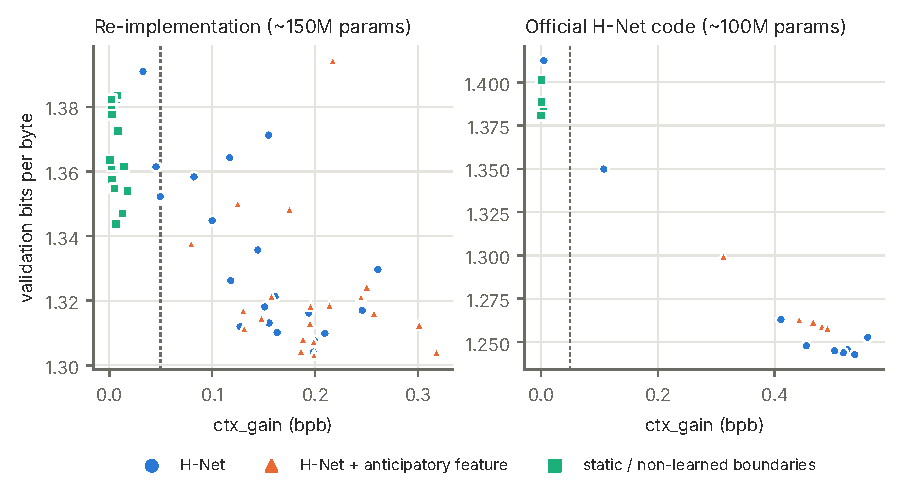
\includegraphics[width=\linewidth]{figures/fig_scatter.pdf}
\caption{Final validation \bpb{} against \ctx{} for every valid run. Static or non-learned
boundaries (fixed stride, fixed stride with H-Net's EMA de-chunking, anticipatory boundaries
without a learned router, and anti-collapse variants) all sit at $\ctx{}\approx0$. Dashed line:
collapse threshold 0.05. Across all runs, $r(\bpb,\ctx{})=-0.82$.}
\label{fig:scatter}
\end{figure}

\begin{table}[t]
\centering
\small
\caption{Main results (final validation \bpb{}, 590M training bytes). ``Collapsed'' = runs with
$\ctx{}\le0.05$. Compression is bytes per chunk (target 4).}
\label{tab:main}
\begin{tabular}{llcccccc}
\toprule
impl. & chunking & seeds & mean \bpb{} & range & \ctx{} range & collapsed & compression\\
\midrule
ours & fixed stride & 2 & 1.369 & 1.357--1.381 & 0.002--0.003 & 2/2 & 4.00\\
ours & fixed stride, 3.6 bytes & 2 & 1.366 & 1.355--1.378 & 0.003--0.004 & 2/2 & 3.60\\
ours & fixed + H-Net de-chunking & 3 & 1.363 & 1.362--1.364 & 0.001--0.002 & 3/3 & 4.00\\
ours & H-Net & 20 & 1.333 & 1.304--1.391 & 0.033--0.261 & 3/20 & 3.64\\
ours & H-Net + anticipatory & 20 & 1.322 & 1.303--1.394 & 0.080--0.318 & 0/20 & 3.56\\
\midrule
official & fixed stride & 3 & 1.390 & 1.381--1.401 & 0.0006--0.0008 & 3/3 & 4.00\\
official & H-Net & 3 & 1.279 & 1.243--1.350 & 0.108--0.537 & 0/3 & 3.49\\
\bottomrule
\end{tabular}
\end{table}

\subsection{Static chunking collapses; H-Net usually does not}

Table~\ref{tab:main} and Figure~\ref{fig:scatter} summarise the main comparison. In our
re-implementation, every run with static boundaries ended with $\ctx{}\le 0.018$ (17/17 runs
across seven configurations), at 1.34--1.38 \bpb{}. The 128-byte-window encoder and decoder
alone form a byte LM of about this quality; the 12-layer main network adds nothing. Matching
H-Net's realised compression with a 3.6-byte stride did not change this, nor did giving fixed
boundaries H-Net's learned EMA de-chunking and straight-through gate (``fixed + H-Net
de-chunking''), which shows that H-Net's de-chunker is not what keeps the main network alive.

The official implementation behaves the same way: official fixed-stride runs reach
1.38--1.40 \bpb{} with $\ctx{}<0.001$, whereas official H-Net reaches 1.24--1.35 \bpb{} with
\ctx{} of 0.11--0.54. When it works, the official model uses its main network far more than our
re-implementation does ($\ctx{}\approx0.5$ vs.\ 0.1--0.3), and is correspondingly better
(1.24 vs.\ $\approx$1.31 \bpb).

\paragraph{H-Net's advantage tracks main-network use.} Across all runs \bpb{} and \ctx{} are
strongly anti-correlated ($r=-0.82$; within the two H-Net arms of our re-implementation alone
$r=-0.52$, where a few poor runs are not collapses). In this regime, the gap between H-Net and
fixed-stride chunking (0.04 \bpb{} ours, 0.11 \bpb{} official) is therefore best described as
the gap between a hierarchy that is used and one that is bypassed.

\begin{figure}[t]
\centering
\begin{minipage}{0.49\linewidth}
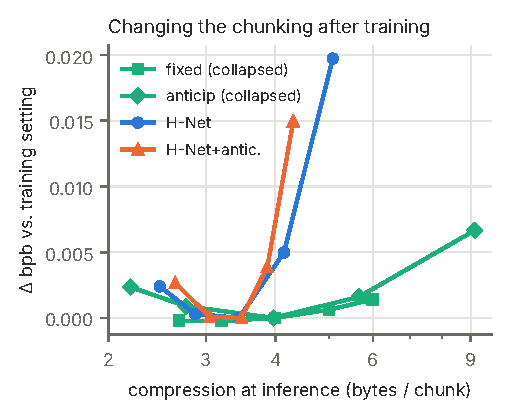
\includegraphics[width=\linewidth]{figures/fig_dial.pdf}
\end{minipage}\hfill
\begin{minipage}{0.49\linewidth}
\caption{Changing the compression of a trained model at inference (ours). Collapsed models
(fixed stride, anticipatory boundaries without a learned router) are almost insensitive to the
chunking: fixed-stride \bpb{} changes by at most 0.0016 between 2.7 and 6.0 bytes per chunk. Models
whose main network is used (H-Net, H-Net + anticipatory) degrade quickly away from their
training compression.}
\label{fig:dial}
\end{minipage}
\end{figure}

\subsection{Collapse is stochastic, even for H-Net}

\begin{figure}[t]
\centering
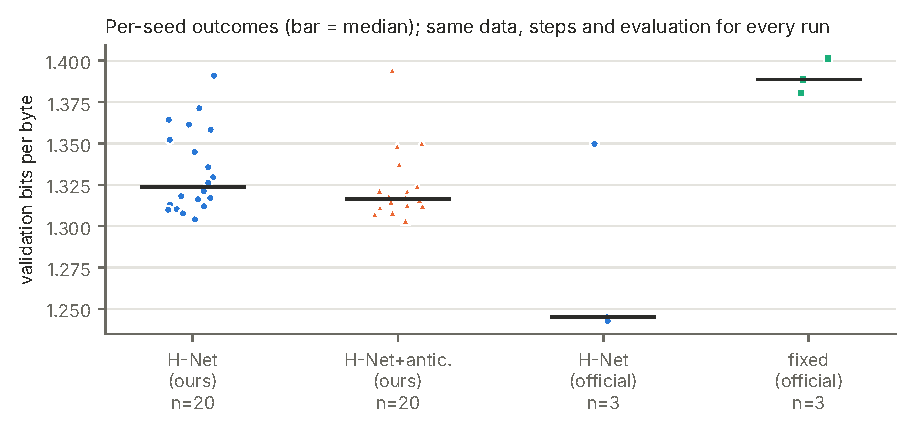
\includegraphics[width=\linewidth]{figures/fig_seeds.pdf}
\caption{Per-seed final \bpb{}. H-Net's outcomes are bimodal-ish: most seeds reach
1.30--1.33 \bpb{}, but several land 0.04--0.06 \bpb{} worse, mostly with a collapsed or partially
collapsed main network. One of three official H-Net seeds ($\ctx{}=0.11$) is 0.1 \bpb{} worse
than the other two ($\ctx{}\approx0.5$).}
\label{fig:seeds}
\end{figure}

With 20 seeds of our re-implementation, H-Net's final \bpb{} ranges from 1.304 to 1.391
(Figure~\ref{fig:seeds}); 3/20 runs collapsed ($\ctx{}\le0.05$) and 7/20 ended above 1.34
\bpb{}. Official H-Net shows the same behaviour on a smaller sample: seeds 1 and 3 reached
1.245 and 1.243 \bpb{} ($\ctx{}=0.50$, 0.54), seed 2 only 1.350 ($\ctx{}=0.11$). Single-seed
comparisons between hierarchical byte LMs can therefore differ by more than the effects being
compared.

%OFFICIAL2_RESULTS%

\subsection{What did not fix collapse}
\label{sec:negative}

\begin{table}[t]
\centering
\small
\caption{Interventions and new chunkers (ours, final \bpb{}). None revived the main network of a
static-boundary model; none beat H-Net.}
\label{tab:negative}
\begin{tabular}{lccc}
\toprule
variant & seeds & mean \bpb{} & \ctx{}\\
\midrule
fixed stride (reference) & 2 & 1.369 & 0.002--0.003\\
\quad + residual warm-up (bypass scaled $0\to1$ over 3k steps) & 2 & 1.350 & 0.013--0.018\\
\quad + LayerNorm on main-network input & 2 & 1.349 & 0.005--0.007\\
\quad + main-network lr $\times0.1$ (instead of $\times0.3$) & 2 & 1.370 & 0.002--0.003\\
anticipatory boundaries, no learned router & 3 & 1.376 & 0.007--0.014\\
\quad + residual warm-up & 1 & 1.373 & 0.009\\
H-Net + residual warm-up (a collapsing seed) & 1 & 1.405 & 0.083\\
\bottomrule
\end{tabular}
\end{table}

\paragraph{Anti-collapse interventions.} Scaling the residual bypass from 0 to 1 over the first
3k steps, normalising the main network's input, or lowering the main network's learning rate
further each left fixed-stride models collapsed (Table~\ref{tab:negative}); the first two
improved \bpb{} by $\approx$0.02 without increasing \ctx{} meaningfully, i.e.\ they helped the
outer networks, not the hierarchy. Residual warm-up also did not rescue an H-Net seed that
collapses without it.

\paragraph{New chunking mechanisms.} Before identifying collapse we designed and evaluated
several mechanisms (definitions in Appendix~\ref{app:chunkers}): continuous integrate-and-fire
chunking \citep{dong2020cif} with exact compression control and three variants;
equal-information chunking (fire when accumulated next-byte surprisal of a detached probe
reaches a running budget); anticipatory chunking (end a chunk where the predictive entropy of the
next byte is high; 66\% of its boundaries fall on spaces or punctuation); H-Net with a realised-surprisal
feature; and fixed boundaries with H-Net's learned de-chunking. None outperformed H-Net, and all
mechanisms without a learned, content-dependent router collapsed when we could measure \ctx{}.

\subsection{Anticipatory routing: fewer collapses, no significant gain}
\label{sec:anticip}

Our most promising variant keeps H-Net's router and adds one feature: the standardised
predictive entropy $\hat H_t$ of the next byte, computed by a small next-byte probe on detached
encoder states (trained by its own cross-entropy, with running normalisation statistics so that
it is causal),
\[
p_t = \mathrm{clip}\Big(\tfrac12\big(1-\cos(W_q h_{t-1}, W_k h_t)\big) + \gamma\,\hat H_t,\; 0, 1\Big),
\]
with learned $\gamma$ (initialised to 0.1). The intent is to call the main network just before
bytes that the encoder finds hard to predict. Over 20 seeds it never collapsed
($\ctx{}\ge0.08$), ended above 1.34 \bpb{} in 3/20 seeds (H-Net: 7/20), and averaged 1.322 vs.\
1.333 \bpb{} for H-Net (Table~\ref{tab:main}). None of these differences is significant: Welch
$t$-test $p=0.15$, Mann--Whitney $p=0.15$, seed-paired $t$-test $p=0.20$, Levene $p=0.19$,
Fisher's exact test on collapse counts $p=0.23$. An interim analysis with 14 vs.\ 16 seeds
showed a significant variance reduction (Levene $p=0.046$) that did not survive the remaining
seeds; one anticipatory seed ended at 1.394 \bpb{} \emph{without} collapsing ($\ctx{}=0.22$). We
report this as a null result with a possible small reliability benefit.

\section{Related work}

Hierarchical and pooled Transformers shorten sequences inside the network
\citep{dai2020funnel,nawrot2021hourglass}; MEGABYTE \citep{yu2023megabyte} and SpaceByte
\citep{slagle2024spacebyte} apply fixed or rule-based patching to bytes, BLT
\citep{pagnoni2024blt} uses entropy-based patches from a separately trained byte LM, and
dynamic token pooling \citep{nawrot2022dtp}, MrT5 \citep{kallini2024mrt5}, H-Net
\citep{hwang2025hnet}, H-Net++ \citep{hnetpp2025} and ByteFlow \citep{byteflow2026} learn where to
segment or merge. Continuous integrate-and-fire \citep{dong2020cif} comes from speech
recognition. The failure mode we describe resembles posterior collapse in VAEs
\citep{bowman2016generating}, where a powerful decoder ignores a latent pathway that the
objective does not force it to use; here the ignored pathway is the chunk-level main network,
and the shortcut is the encoder-to-decoder residual.

\section{Limitations}

Our models are small (100--150M parameters) and trained on 590M bytes, far below the scale of
the H-Net paper; the residual shortcut may matter less when encoder and decoder are relatively
weaker or training is longer. We use one dataset, one-stage hierarchies, and target compression
4. Official-code results use 3 seeds per arm (plus the additional runs in
Section~\ref{sec:mech}); our re-implementation differs from the official code (Transformer
instead of Mamba-2 encoder/decoder) and is weaker in absolute terms. \ctx{} measures dependence
on the main network's chunk-specific content under mean replacement; it is a diagnostic, not a
complete account of what the main network computes.

\section{Conclusion}

In hierarchical byte-level LMs the main network can be bypassed without any visible failure in
the loss. At our scale this happened in every model with static chunk boundaries, in both a
re-implementation and the official H-Net code, and occasionally to H-Net itself; H-Net's
advantage over fixed chunking was largely the difference between a used and an unused
hierarchy. We recommend that work on hierarchical byte-level models report \ctx{} or a similar
bypass check, test sensitivity to the chunking at inference, and report multiple seeds.

\paragraph{Reproducibility.} Code, run configurations, all per-run results and the scripts that
produce every table and figure are in the accompanying repository (\texttt{research/dcbench}).

\bibliographystyle{plainnat}
\bibliography{refs}

\appendix
\section{Chunking mechanisms}
\label{app:chunkers}
All mechanisms share the encoder, main network, decoder and residual path; only down-sampling
and up-sampling differ. Byte $t$ may only read chunks completed at or before $t$.
\begin{itemize}
\item \textbf{Fixed}: a boundary every $N$ bytes (fractional $N$ allowed via $\lfloor t/N\rfloor$).
\item \textbf{H-Net} \citep{hwang2025hnet}: cosine router, EMA de-chunking, straight-through
  confidence, load-balancing loss (Section~\ref{sec:background}).
\item \textbf{Integrate-and-fire (IF)}: each byte emits $a_t\in(0,1)$, $C_t=\sum_{s\le t}a_s$; a chunk
  fires when $C_t$ crosses an integer, so the number of chunks is exactly $\lfloor\sum a_t\rfloor$.
  The chunk vector is the $a$-weighted average of its bytes (\texttt{if}) or, in the forward pass,
  the state of the firing byte with gradients through the pooling weights (\texttt{if\_last}).
\item \textbf{Equal-information}: $a_t=\min(1,s_t/B)$ with $s_t$ the surprisal of byte $t$ under a
  detached next-byte probe and $B$ a running budget $\approx N\cdot\mathbb{E}[s]$.
\item \textbf{Anticipatory boundaries}: boundary at $t$ when the probe's predictive entropy of byte
  $t{+}1$ exceeds a threshold adjusted online to keep the boundary rate at $1/N$.
\item \textbf{H-Net + realised surprisal / + anticipatory}: H-Net's router logit plus $\gamma$ times
  a standardised surprisal (of $x_t$) or predictive-entropy (of $x_{t+1}$) feature.
\item \textbf{Fixed + H-Net de-chunking}: fixed boundaries, but H-Net's learned $p$ drives the EMA
  de-chunking and the straight-through gate.
\item \textbf{Random} (official code): boundaries drawn independently with probability $1/N$.
\end{itemize}

\section{Earlier experiments}
\label{app:earlier}
A CPU study (12.5M parameters, 6.5\,MB of English text, 1{,}500 steps) and three initial GPU
waves preceded the results above. In the CPU study no mechanism separated from fixed-stride
chunking beyond seed noise ($\approx$0.01 \bpb), and an early single-seed ``win'' of
integrate-and-fire chunking (0.09 \bpb) on a distribution-shifted validation split did not
replicate on a clean split. The first three GPU waves used full causal attention in the
encoder and decoder and a main-network learning rate of $10^{-3}$; a compression sweep showed
\bpb{} unchanged to four decimals between 2.7 and 6 bytes per chunk, which led us to the
\ctx{} diagnostic. We exclude those waves from all conclusions.

\section{Use of AI assistance}
The experiments, analysis code and a first draft of this paper were produced with the help of an
AI coding agent operating under the authors' direction; all numbers are generated by the
scripts in the repository from the logged runs.

\end{document}
